%%%%%%%%%%%%%%%%%%%% BACKGROUND SECTION %%%%%%%%%%%%%%%%%%%%%%%%%%
\section{Background}
\label{sec:back}

In this section, we first give a brief overview of the distance vector and then describe the count-to-infinity problem.

\subsection{Distance Vector Algorithm}

Distance vector is a single source shortest paths algorithm that is both distributed and asynchronous.  The input of the algorithm is a graph 
with indexed nodes and weighed edges.  The output of the algortihm is 
least cost paths from every node to every other node in the graph. 

Path cost computation relies on nodes sharing their least path costs with their neighbor nodes.  
Path costs are only shared when a new least cost path is discovered. To begin, nodes set their unknown path costs to $\infty$.  Upon the discovery of 
a new least cost path, this cost is shared with each neighbor node.  Each neighbor then determines if this new path cost results in its own new least 
cost path. If so, this update is shared with each of the node's neighbors.  This process iterates until 
there are no routing updates to send.  In this way the algorithm naturally converges. (e.g., there is no outside source that terminates the path cost computation). 

Distance vector computation is distributed because multiple nodes communicate to find least cost paths; a node receives messages, 
performs a computation, and then (potentially) distributes the resulting calculation. 
Also distance vector is asynchronous because nodes do not need to operate at the sample clock rate. %a node's computation takes place without coordination.

Each node represents path costs in a routing table.  Conceptually, there is a column for each destination and a row for every neighbor.  
Least-cost paths are computed as follows. Let $d_x(y)$ be the value of the least cost path from node $x$ to node $y$ and $min_v$ is taken over all 
of $x$'s neighbors. The following formula determines how $x$ computes its least cost path to $y$: 

\begin{eqnarray}
 d_x(y) &=& min_v\{c(x,v) + d_v(y)\} 
\end{eqnarray}

Consider the example taken from \cite{KuroseRoss04} and shown in Figure \ref{fig:dv-example}. The graph consists of $3$ nodes: $x$, $y$, and $z$. 
Each column in Figure \ref{fig:dv-example} 
represents a single timestep. For ease of exposition, the example considers the case when nodes compute path costs in a synchronous manner. It is important 
to note that this is not a constraint imposed by the algorithm. Correctness is preserved when nodes operate asynchronously. 

In the first timestep, each node
is only aware of its $1$-hop paths to each node in the graph.  For this reason, only a single routing table row is populated with non-$\infty$ 
values.  For example, $x$'s distance vector is $[0,2,7]$: $x$ can route to $x$ with cost $0$, to $y$ with cost $2$, and to $z$ with cost $7$.  
For each node, the distance vectors are all new least cost paths, so each node sends its distance vector to its neighbors.  
These messages are depicted as arrows between routing tables.

%Since for each node the $1$ hop costs represent new least cost paths, messages are sent to each neighbor including these cost values. In Figure \ref{fig:dv-example} the arrows between nodes represent the messages.

%\begin{figure}[hT]
%        \centering
%		  \includegraphics[scale=0.80]{figs/dv-example.pdf}
%			\caption{Distance vector example}
%			\label{fig:dv-example}
%\end{figure}


In the second timestep, each node receives a message from its neighbors with their least cost vectors. A node uses these values to update its distance vector. 
For example, node $x$ carries out the following sequence of steps:

\begin{enumerate}

	\item $y$'s and $z$'s distance vector are added to row $2$ and $3$ of $x$'s routing table, respectively. 
	\item Row $1$ is computed using equation $(1)$. Let $D_x(y)$ represent $x$'s distance to $y$ and likewise, $D_x(z)$, $x$'s distance to $z$.  
	$x$'s distance vector is computed as follows:

	\begin{eqnarray*}
		 D_x(x) &=& 0 \\
		 D_x(y) &=& min[c(x,y) + D_y(y),c(x,z) + D_z(y)] \\
		 		  &=& min[2+0,7+1]=2 \\ 
		 D_x(z) &=& min[c(x,z) + D_z(z),c(x,y) + D_y(z)] \\
		 		  &=& min[7+0,2+1]=3 \\ 
	\end{eqnarray*}

	\item $x$ has a new least cost path to $z$ and therefore sends its distance vector to $y$ and $z$. 
\end{enumerate}

$y$ and $z$ carry out the same sequence of steps; they recompute their distance vectors and 
if their distance vectors change they send updates their neighbors.  Notice that $y$'s distance vector does not change in the second timestep, therefore
it does not send any updates. 

In the third timestep, the distance vectors are unchanged.  No messages are sent and each node enters a quiescent state.

\subsection{Count-to-Infinity Problem}
Because nodes running the distance vector algorithm are only aware of the costs to their neighbors and their neighbor's least cost paths, nodes may attempt to 
use network paths that do not actually exist. This is known as the count-to-infinity problem. The count-to-infinity problem arises when either link
costs change or when a node is removed from the network (typically because of an unrecoverable failure).

We explain the count-to-infinity problem by way of example. Consider the example in Figure \ref{fig:count-inf}  
and for simplicity let $v_2$ be the only destination of interest.  At time $t_0$ (top figure) both $v_0$ and $v_1$ use the $v_1 - v_2$ link to route to $v_2$. 
Then at some point between $t_0$ and $t_i$ the $v_1 - v_2$ link cost changes to $1006$. This occurrence is reflected in the lower graph.  At this point, 
$v_1$ determines its new
least cost path to $v_2$ is through $v_0$ with cost $20$, unaware that $v_0$ assumes the $v_1-v_2$ link cost is $10$.  $v_1$ then advertises its new least cost path.  
$v_0$ applies this update and determines its new least cost to $v_2$ is $25$.  This process repeats itself until $v_0$'s cost to $v_2$ through $v_1$ exceeds $1000$,
requiring $194$ messages! At this point, the $v_0 - v_2$ link is used in favor of $v_1 - v_2$.  

The previous example shows that the count-to-infinity problem can be costly. Thus when designing recovery algorithms we would like to avoid such scenarios.

%%%%%%%%%%%%%%%%%%%%%%%%%%% COMMENT %%%%%%%%%%%%%%%%%%%%%%%%%%%%%%%%%%%%%%%%%
\begin{comment}
\begin{figure}

\begin{center}

\underline{Network at time $t_0$}
\vspace{0.2cm}

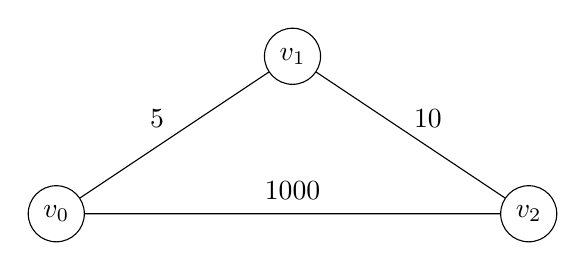
\begin{tikzpicture}[scale=2]
\tikzstyle{every node}=[draw,shape=circle];
	\path (0:1.5cm)    node (v0) {$v_2$};
	\path (90:1cm)   node (v1) {$v_1$}; 
	\path (180:1.5cm)   node (v2) {$v_0$}; 

	\draw (v0) -- (v1)
			(v0) -- (v2)
			(v1) -- (v2);
\tikzstyle{every node}=[];
	\path (90:0.15cm)  node (vt) {$1000$}; 
	\path (35:1.05cm)  node (vt) {$10$}; 
%	\path (35:1.35cm)  node (vt) {$\nearrow$}; 
%	\path (35:1.65cm)  node (vt) {$1006$}; 
	\path (145:1.05cm)  node (vt) {$5$}; 

\end{tikzpicture}


\vspace{0.2cm}
$ \Big\Downarrow $
\vspace{0.2cm}

\underline{Network at time $t_i$}
\vspace{0.2cm}

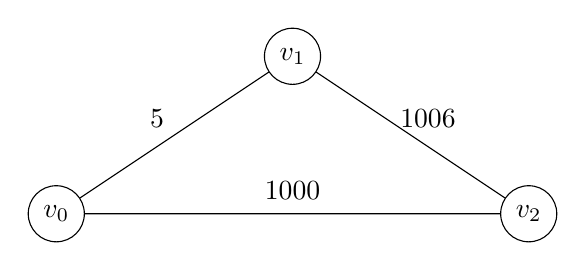
\begin{tikzpicture}[scale=2]
\tikzstyle{every node}=[draw,shape=circle];
	\path (0:1.5cm)    node (v0) {$v_2$};
	\path (90:1cm)   node (v1) {$v_1$}; 
	\path (180:1.5cm)   node (v2) {$v_0$}; 

	\draw (v0) -- (v1)
			(v0) -- (v2)
			(v1) -- (v2);
\tikzstyle{every node}=[];
	\path (90:0.15cm)  node (vt) {$1000$}; 
	\path (35:1.05cm)  node (vt) {$1006$}; 
	%\path (35:1.35cm)  node (vt) {$\nearrow$}; 
	%\path (35:1.65cm)  node (vt) {$1006$}; 
	\path (145:1.05cm)  node (vt) {$5$}; 

\end{tikzpicture}

\end{center}


\caption{Count-to-infinity example. Between time $t_0$ and $t_i$, link $v_1 -v_2$ cost changes from $10$ to $1006$. The top graph shows 
  the state of the network at time $t_0$ and the lower graph depicts the network at time $t_i$.}
\label{fig:count-inf}
\end{figure}


\end{comment}
%%%%%%%%%%%%%%%%%%%%%%% END COMMENT %%%%%%%%%%%%%%%%%%%%%%%
 





%%%%%%%%%%%%%%%%%%%%%%% COMMENTED OUT FIG %%%%%%%%%%%%%%%%%%%%%%%
\begin{comment}
\begin{figure}
	\label{fig:count-inf}
	\begin{center}

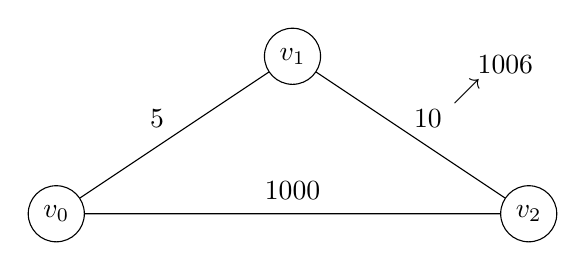
\begin{tikzpicture}[scale=2]
\tikzstyle{every node}=[draw,shape=circle];
	\path (0:1.5cm)    node (v0) {$v_2$};
	\path (90:1cm)   node (v1) {$v_1$}; 
	\path (180:1.5cm)   node (v2) {$v_0$}; 

	\draw (v0) -- (v1)
			(v0) -- (v2)
			(v1) -- (v2);
\tikzstyle{every node}=[];
	\path (90:0.15cm)  node (vt) {$1000$}; 
	\path (35:1.05cm)  node (vt) {$\cancel{10}$}; 
	\path (35:1.35cm)  node (vt) {$\nearrow$}; 
	\path (35:1.65cm)  node (vt) {$1006$}; 
	\path (145:1.05cm)  node (vt) {$5$}; 

\end{tikzpicture}
\end{center}

\end{figure}
\end{comment}

